\section{Synchronization Design}
The purpose of the synchronization is to create a local database on an Android device that can be kept in synchronization with the central database. The idea behind the synchronization is that many different Android devices should be able to access information about the same users. For this to work correctly, the data on different Android devices should be the same, otherwise the concept of a central database that stores all data will be moot. This means that the database on the Android device will include the same exact data that the central database includes, and as such the two databases must have the same tables. In addition to downloading data from the central database, an Android device will be able to create data itself. This data can then be uploaded to the central database to be kept in synchronization with many different devices.

The application that will synchronize the data between Android devices and the central database will run on the Android devices, and will thus be written in Java.

\subsection{The Application}
The application Puddle is meant to be a smaller prototype version of the OasisLib application from previous years. Unlike OasisLib, Puddle is not a library that can be accessed by other Android applications on a device. The database that Puddle creates can therefore only be accessed by the Puddle application itself.

\begin{figure}[hptb]
    \begin{center}
    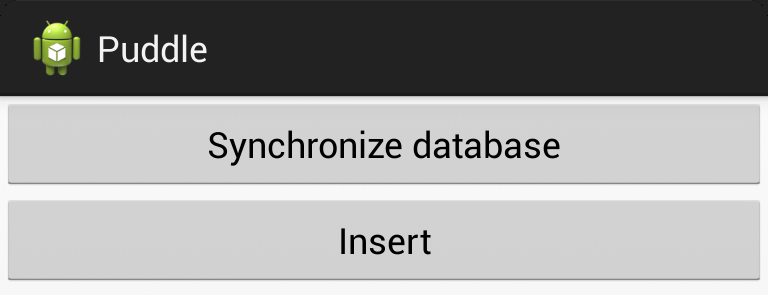
\includegraphics[width=0.8\textwidth]{img/puddle-app.png}
    \caption{Overview of the Puddle Android application.}
    \label{fig:puddle_app}
    \end{center}
\end{figure}

\autoref{fig:puddle_app} shows the Puddle application as it launches on an Android device. Puddle has two buttons, one for synchronizing with the central database, and one for inserting information into the local database. Puddle synchronizes manually with the central database, and needs to be launched manually. To synchronize, press the synchronize button, and Puddle will upload changes made to the local database, and then download from the central database. When the insert button is pressed, it inserts predefined information from the MainActivity class into the local database.

\subsection{Creating a Local Database}
Before it is possible to save to a local database on an Android device, it must first be created. Android only has native support for the SQLite to create databases, SQLite is therefore used for the local database in Puddle. %Kilder?
The local database is not created until it is needed. This means that the local database will not be created until the synchronization with the central database is started. The local database is not deleted, however, unless it is actively requested. On subsequent synchronizations there is no need to create the local database again.

\subsection{Uploading \& Downloading Changes}
Changes made on an Android device should not be deleted when the two databases are synchronized. To avoid it, the changes are first uploaded to the central database, before new data from the central database is downloaded to the Android device. This has the unfortunate side effect that changes made to the central database will be lost. We have decided that changes made on Android devices will always supersede changes made to the central database.

Before uploading changes made on the Android device, the changes must be found. To find these changes, a table has been added to the local database that does not exist in the central database. This table contains a timestamp with the time of the most recent synchronization with the central database. An additional attribute is added to all tables in the local database. This attribute also contains a timestamp, but this timestamp is updated when the table is inserted or changed. Every table that has a newer timestamp than the last synchronization, has been changed or added after the last synchronization. These will be uploaded to the central database at the next synchronization. If there are no changes, this step will be skipped.

When synchronizing with the central database, everything will be downloaded to the local database. To do this, each table in the central database will be queried, downloaded and inserted into the corresponding table in the local database with a timestamp added. Every time the databases are synchronized, the entire central database is downloaded and overwrites the local database.

\subsection{Design Limitations}
Due to design choices in both the central and local database there are multiple limitations of the current design of the synchronization.

One of these limitations is that an update to the central database will be overwritten by an update from an Android device, even if the update to the central database is newer than the update on the Android device. This is a direct consequence of timestamps only being added on the local database. If timestamps were to be added to the central database as well, it would be possible to compare timestamps before inserting updates into the central database. This would make it possible to always keep the most recent change.

Another limitation is that the entire database is downloaded to each individual Android device. In a real world scenario, it would be smarter to limit the download to users and profiles associated with the device and download data for new users as needed. The current solution does not scale very well, and would cause the local database to grow unnecessarily large if the system were to be widely used. This problem could be avoided if the central databases included timestamps on all additions and updates. This way, Puddle could synchronize only the changes newer than last synchronization. %Mention data patches?

A third limitation is that the local SQLite is unencrypted, and can be accessed by anyone who wishes to. This is of course a security risk if the system were to be used in a production environment, because anyone can get access to sensitive user data and more.